% !TEX root =/main.tex
\chapter{Synchronization}
\section{Motivation}
If we run different threads in a program and they execute in parallel, this means that they might try to access data at the same time. What happens if Thread 1 tries to read variable A at the same time as Thread 2 tries to write to it? we can't know which one will access the data first.

\section{The Critical Section problem}
When writing syncronized code we create a ''critical section'' in which only one thread are allowed to execute at a time, even if the critical sections are different only one thread can be in one of them at a time.
\begin{figure}[H]
	\centering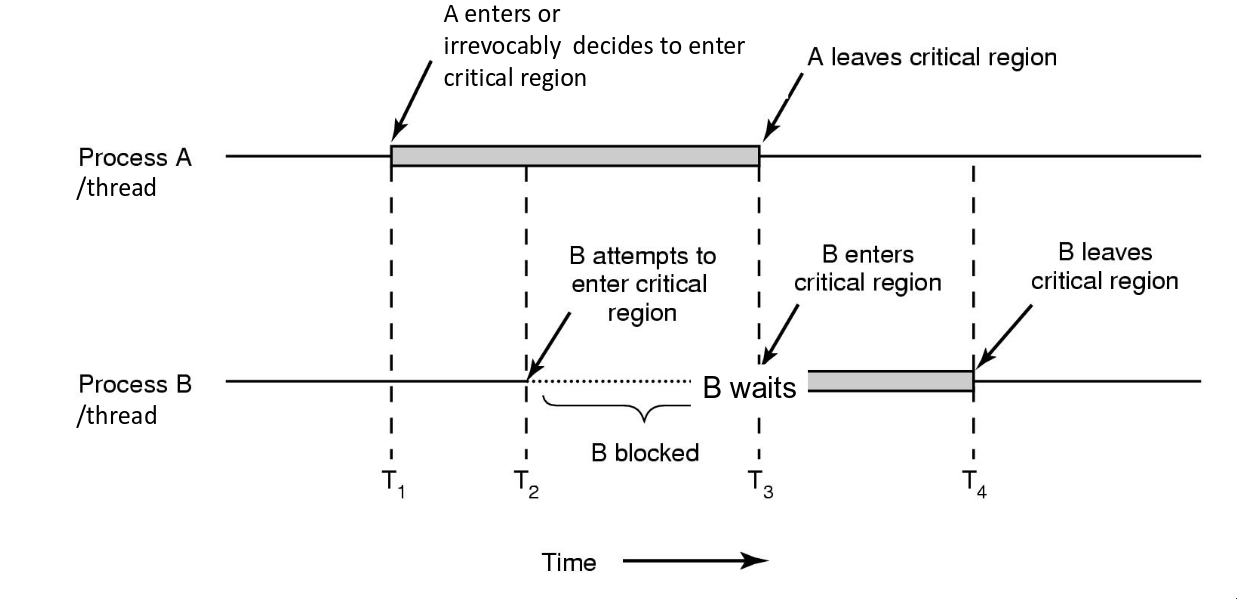
\includegraphics[width=.5\textwidth]{images/critical_section_desire.png}
	\caption{The desired outcome of the critical region problem.}
	\label{fig:critical_section_problem}
\end{figure}
We need to solve the problem of critical section in such a way that: only one thread at a time is allowed to execute a critical section; other threads can enter their critical sections in bounded time when no process is currently in its critical section; no thread will be starved, endlessly waiting for its turn of executing a critical section.

\subsection{Check-competition approach}
\begin{figure}[H]
	\centering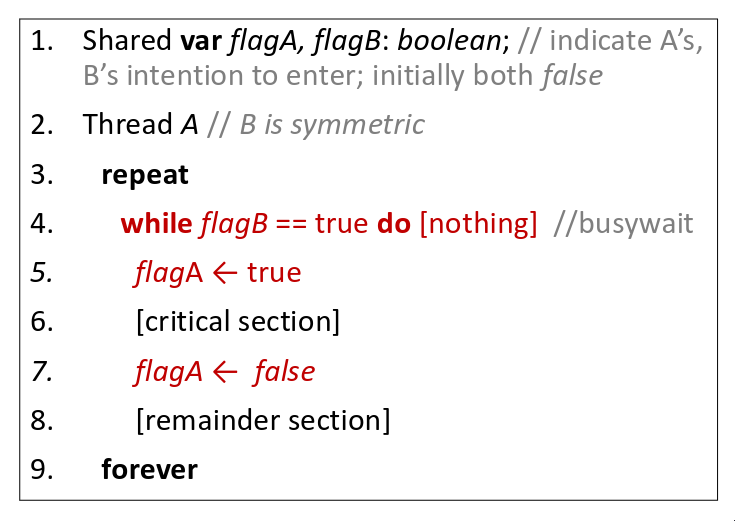
\includegraphics[width=.5\textwidth]{images/check_competition.png}
	\caption{The check-competition approach to critical section problem.}
	\label{fig:check_competition}
\end{figure}
One approach to the critical section problem is the Check-competition approach (see \ref{fig:check_competition}), this however fails at the mutual exclusion property, since several threads can manage to execute its line 4 before any thread manages to execute its line 5, blocking threads from executing line 4.

\subsection{The check-order / after-you approach}
\begin{figure}[H]
	\centering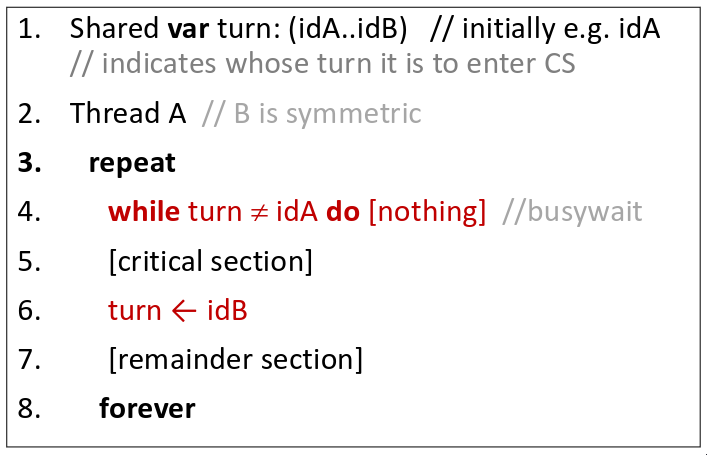
\includegraphics[width=.5\textwidth]{images/check_order.png}
	\caption{The check-order approach to critical section problem.}
	\label{fig:check_order}
\end{figure}
Another approach is called check order (see \ref{fig:check_order}) and lets the threads take turn executing their critical section, instead waiting for their turn instead of deciding themselves when it's their time to execute. A problem with this however is starvation, since if the thread before never enters its critical section, all following threads will be stuck waiting forever.
\subsection{Peterson’s Algorithm}
If we however combine the outcomes of these two approaches, we get a solution that works, Peterson's algorithm is this solution (see \ref{fig:peterson})
\begin{figure}[H]
	\centering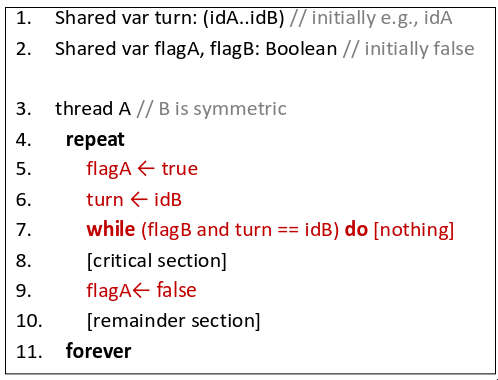
\includegraphics[width=.5\textwidth]{images/peterson_algo.png}
	\caption{Peterson's algorithm, a working solution to the  critical section problem.}
	\label{fig:peterson}
\end{figure}
\section{Synchronization and hardware support}
%To make sure nothing else executes while we are in the critical section, we can disable interrupts while executing it.
One hardware solution to the mutual exclusion problem is to just disable interrupts while in the critical section. There are however some problems with this.
\begin{itemize}
	\item If we use a multiprocessor system, the threads running on different cores might still cause issues.
	\item If we run on a single-core system, nothing else can execute, meaning everything else will function.
\end{itemize}

\subsection{Read-Modify-Write instructions}
We can use an instruction called TestAndSet which atomically tests a value, and sets its value to true. Using this we can create locks which only one process are able to pass through.

\begin{figure}[H]
	\centering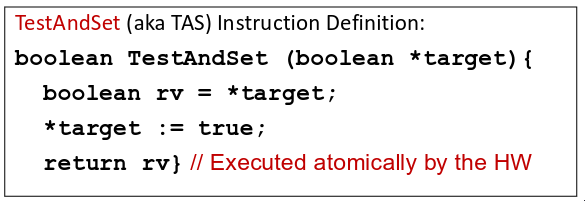
\includegraphics[width=.5\textwidth]{images/test_and_set.png}
	\caption{Pseudo code for what Test and set does.}
	\label{fig:tas}
\end{figure}

\begin{figure}[H]
	\centering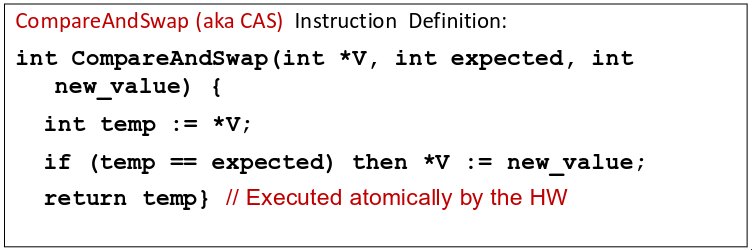
\includegraphics[width=.5\textwidth]{images/compare_swap.png}
	\caption{Pseudo code for what compare and swap does.}
	\label{fig:cas}
\end{figure}

\subsection{Reflection on busy-waiting}

Right now all the solutions are using busy-waiting, meaning they actively check for when they can continue. While this is a simple solution, it consumes computing resources without any reason to, it might starve , and deadlocks might happen if the thread waiting to use its critical section has higher priority than the one in a critical section, meaning the busy-waiting thread gets to execute its wait while the thread it waits for is not allowed to execute until the waiting thread has terminated.

\section{Semaphores}

\section{Other techniques}
